\documentclass[conference]{IEEEtran}
\IEEEoverridecommandlockouts
% The preceding line is only needed to identify funding in the first footnote. If that is unneeded, please comment it out.
\usepackage{cite}
\usepackage{amsmath,amssymb,amsfonts}
\usepackage{algorithmic}
\usepackage{graphicx}
\usepackage{textcomp}
\usepackage{xcolor}
\def\BibTeX{{\rm B\kern-.05em{\sc i\kern-.025em b}\kern-.08em
    T\kern-.1667em\lower.7ex\hbox{E}\kern-.125emX}}
\begin{document}

\title{Modeling and simulation of Power Consumption on Heterogenous CPU Cores under varying workloads and operating conditions\\

}

\author{\IEEEauthorblockN{Atharv Arun Desai}
\IEEEauthorblockA{\textit{Department of CSA} \\
\textit{Indian Institute of Science (IISc)}\\
Bangalore, India\\
atharvarun@iisc.ac.in}
\and
\IEEEauthorblockN{Boul Chandra Garai}
\IEEEauthorblockA{\textit{Department of CSA} \\
\textit{Indian Institute of Science (IISc)}\\
Bangalore, India \\
chandraboul@iisc.ac.in}
\and
\IEEEauthorblockN{Himanshu Srivastava}
\IEEEauthorblockA{\textit{Department of CSA} \\
\textit{Indian Institute of Science (IISc)}\\
Bangalore, India\\
himanshusriv@iisc.ac.in}
\and
\IEEEauthorblockN{Vaisakh P S}
\IEEEauthorblockA{\textit{Department of CSA} \\
\textit{Indian Institute of Science (IISc)}\\
Bangalore, India\\
vaisakhp@iisc.ac.in}
}

\maketitle

\begin{abstract}
    This document serves as phase-1 report for E0-240 - Modeling and Simulation course project delivery. The main objective of this project is to apply concepts learned in E0-240 course in to Modeling and simulation of a real-world system, which in this case is Multi-core, Heterogenous CPU. This project, will focus on developing a Power Consumption Model for simulated Full-System \cite{8718630} under varying workloads. This model will be developed taking in consideration various operating conditions of the CPU such as Dynamic Frequency Scaling, Heterogenous Cores \cite{arm-big.little-whitepaper}
\end{abstract}

\begin{IEEEkeywords}
    Modeling, simulation, heterogenous CPU cores, power consumption
\end{IEEEkeywords}

%% ---------------------------------------------------------------------------------------------------------
%% Background 
%%    - Motivation behind the work
%%    -  any technical background (any special definition/technology which is a required knowledge to 
%%       understand the rest of the document)
%%    - existing work in the domain etc. 
\section{Background}
%% ---------------------------------------------------------------------------------------------------------
    \par Power consumption is one of the key performance indices of any embedded or mobile device which operate of power budget, as this directly impacts on user experience and usability of any such devices. Hence, the need for accurate power models in simulation environment has increased as well, to enable designer and manufacturers to measure the impact of any new functionality or optimization that is being prototyped. Insights from such models, will allow all key stakeholders in an embedded product development arena for evaluation without waiting hardware fabrication and rollout, there by saving resources and investment.

    \par One of the main motivations for this project is the top-down power modeling approach\cite{Reddy2017EmpiricalCP} that utilized Performance Monitoring Counters(PMCs) in an actual hardware along with overall power consumption data to develop an empirical power model in Gem5 simulator\cite{8718630}. The average error achieved by this approach is claimed to be less than 6\%. We will further explore in to additional enhancement over this said approach by factoring in additional CPU performance metrics.

%% ---------------------------------------------------------------------------------------------------------
%% Covers Methodology, development strategy, data gathering approaches etc.
\section{Methodology}
%% ---------------------------------------------------------------------------------------------------------
    \par As mentioned in previous work \cite{Reddy2017EmpiricalCP}, a similar method is followed in developing a Top-down Power model that will be integrated in to Gem5. ODROID-XU4\cite{odroid-xu4} Big-Little development board is chosen as first target for experimentation, data gathering and validation efforts. An overview of this hardware is show in Figure. \ref{fig-odroid-hwoverview}. ODROID-XU4 offers minimalistic development platform with a Samsung Exynos 5422 Octa ARM Cortex™-A15 Quad 2GHz and Cortex™-A7 Quad 1.3GHz CPUs, with a 2GB LPDDR3 RAM operating at 933MHz stacked along with CPU package. Both Cortex-A15 and Cortex-A7 cores has 32KB Instruction and Data caches each. For L2 cache, the Cortex-A15 and Cortex-A7 cores makes use of 2MB and 512 KB respectively.

    \begin{figure}[bh]
        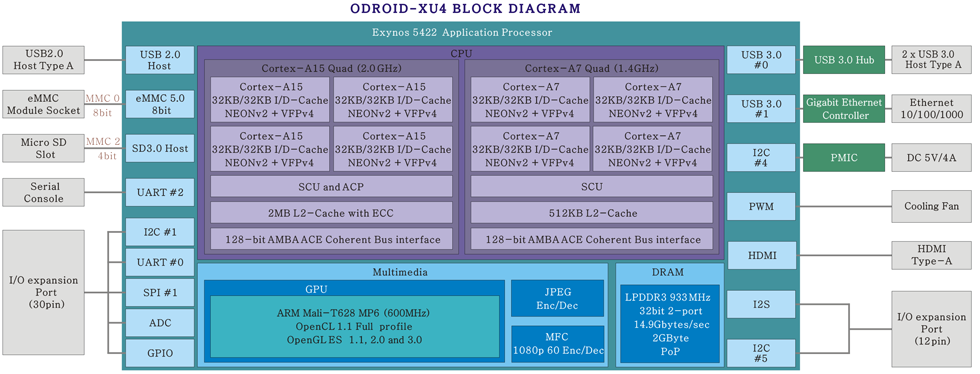
\includegraphics{rsrc/201506191222574523.png}
        \caption{ODroid XU4 board overview}
        \label{fig-odroid-hwoverview}
    \end{figure}

    \subsection{Modeling and Development Strategy}
        \par Simulation of the ODROID-XU4/Exynos5422 will be integrated in to Gem5, that would closely resemble its CPU operating parameters. A SmartPower3 \cite{odroid-smartpower3}, power monitor unit will be used along ODROID-XU4 as represented in Figure. \ref{fig-Experiment-setup}, to measure overall power consumption on the hardware, while most of the peripheral modules on it will be kept to reduce any variation or impact on the measured data. In addition, the perf\cite{2015137} is used to gather PMC data-points. A summary of data-points being gathered for this modeling exercise is listed in Table \ref{Power-Perf-data-gathered}. These data-points are sampled at an interval of 100ms from both perf and SmartPower2 modules.

        \begin{figure}[t]
            \centering
            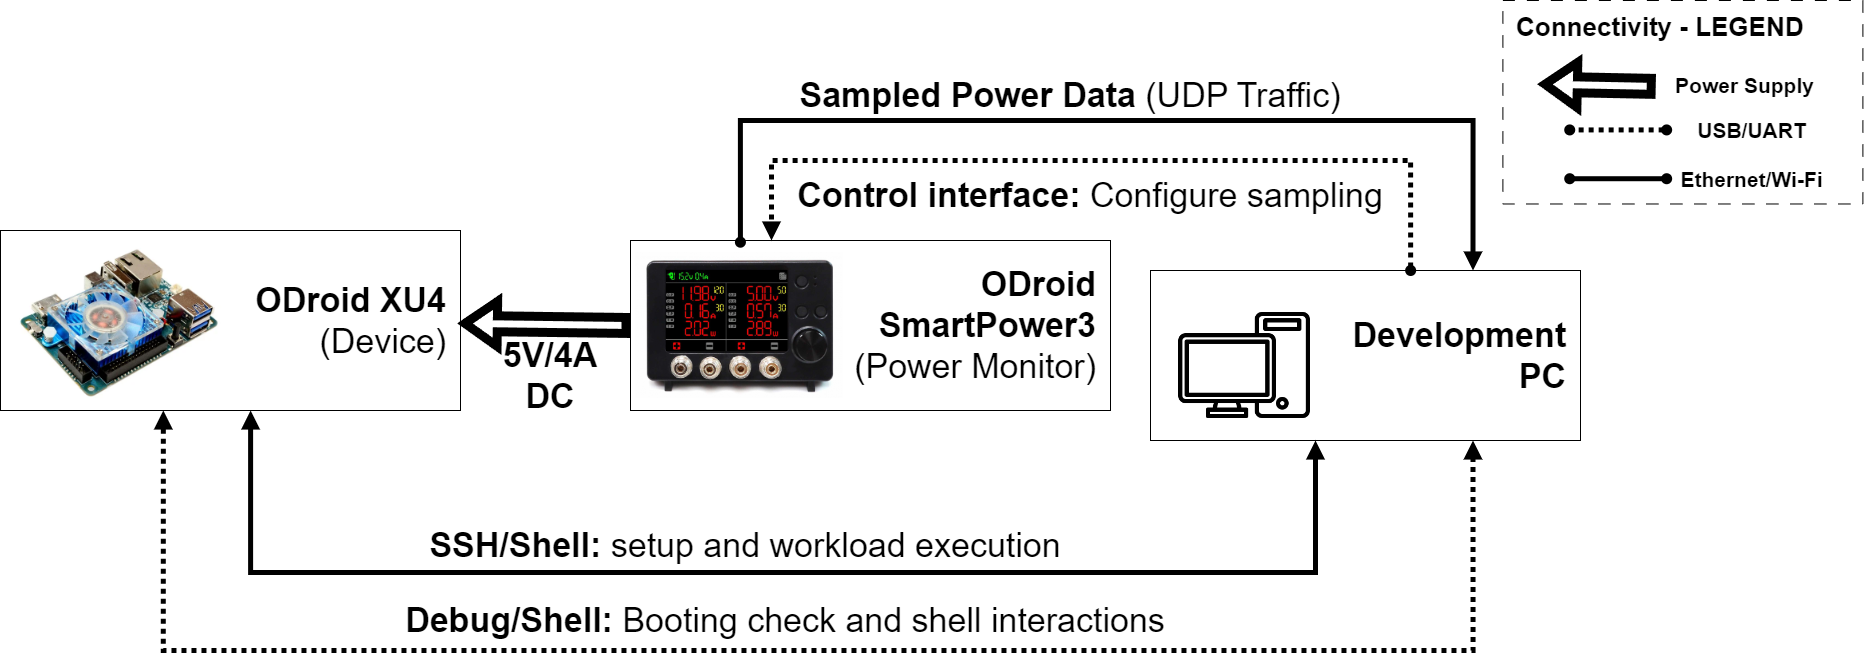
\includegraphics[width=0.48\textwidth]{rsrc/Experiment-setup.drawio.png}
            \caption{Experiment setup for power data gathering from ODROID-XU4\cite{odroid-xu4} hardware}
            \label{fig-Experiment-setup}
        \end{figure}

        \begin{table}[htbp]
            \caption{Power and Performance Feature gathered from mentioned experiment setup}
            \begin{center}
                \begin{tabular}{|p{1.8cm}|p{1.5cm}|p{3.7cm}|}
                    \hline
                    \textbf{Statistics}&\multicolumn{2}{|c|}{\textbf{Feature details}} \\
                    \cline{2-3} 
                    \textbf{Type} & \multicolumn{1}{|c|}{\textbf{\textit Source}} & \multicolumn{1}{|c|}{\textbf{\textit Details}} \\
                    \hline
                    CPU Clock Cycles  & perf\cite{2015137}  & CPU cycles, us cycles, instructions, CPU frequency, CPU idle state statistics \\
                    \hline
                    Instruction Branches  & perf & Branch instruction and speculative operation statistics \\
                    \hline
                    Caches   & perf  & Data/Instruction cache references, misses at L1, Last-Level-Cache levels  \\
                    \hline
                    Board Level Power consumption & SmartPower3\cite{odroid-smartpower3} & Current, Power drawn from power supply. \\
                    \hline
                    Misc. Performance  & perf  & CPU Migrations, Context switches, Virtual memory \\
                    \hline
                \end{tabular}
                \label{Power-Perf-data-gathered}
            \end{center}
        \end{table}

        \par A set of preliminary workloads that would induce resource load for CPU and memory will be executed on the ODROID-XU4 device, while the power consumption and PMC data are simultaneously recorded. Few of the workloads that are being considered as listed in Table \ref{Workload-listing}. As of now, a total of 5 workloads have been employed. Furthermore, integration of SPEC2017 will allow inclusion of up to 43 feasible benchmarks to improve quantity of data.

        \begin{table}[htbp]
            \caption{List of workloads being used for data gathering and validation}
            \begin{center}
                \begin{tabular}{|c|p{4cm}|c|}
                    \hline
                    \textbf{Workload}&\multicolumn{2}{|c|}{\textbf{Workload details and status  of integration}} \\
                    \cline{2-3} 
                    \textbf{Type} & \multicolumn{1}{|c|}{\textbf{\textit Workloads}} & \textbf{\textit{Status}} \\
                    \hline
                    Stress Test & stress command \cite{linux-stress-testing} & $\checkmark$ \\
                    \hline
                    Video Encoding & ffmpeg encode \cite{linux-stress-testing} & $\checkmark$ \\
                    \hline
                    File Compression & gzip, bzip2, xz on complex datasets \cite{compression-benchmarking} & $\checkmark$ \\
                    \hline
                    Benchmark Suite & SPEC2017 CPU Benchmarks \cite{10.1145/3185768.3185771} & Planned \\
                    \hline
                \end{tabular}
                \label{Workload-listing}
            \end{center}
        \end{table}

%% ---------------------------------------------------------------------------------------------------------
\section{Phase-2 Progress}
%% ---------------------------------------------------------------------------------------------------------
    \par So far, team has completed, ramping up in to Gem5 simulator and its internals. In terms of actual hardware data gathering, the experiment setup shown in Figure \ref{fig-Experiment-setup} is established and data gathering of integrated workloads mentioned in Table \ref{Workload-listing} on ODROID-XU4 hardware is also completed as well.

    \par Mathematical modeling with the data obtained is progressing, we are expecting to arrive at the empirical mathematical model soon and will be integrated in to the simulated Gem5 Exynos5422 instance for validation and further refinement.

%% ---------------------------------------------------------------------------------------------------------
\section{ Discussion on Phase-2 outcomes}
%% ---------------------------------------------------------------------------------------------------------
    \par In terms workload execution, these workloads can get executed on any of the available CPU cores in Big and Little clusters, thereby greatly influencing the runtime performance and the power consumption behavior of the same workload. This can be a problem on accuracy of the empirical model being developed. In order avoid the same, we will be restricting execution of workloads to specific code by making use of affinity management primitives available in Linux.

    \par The variations in power consumption seems to be also being influenced by the CPU Dynamic Clock Performance Governors \cite{10.1145/3167132.3167198} and associated modules in Linux Performance management. We may investigate in to the influence of one or more governors on the power consumption and integrate the same in to the empirical model being developed.

%% ---------------------------------------------------------------------------------------------------------
\section{Next Step}
%% ---------------------------------------------------------------------------------------------------------
    \par For integrating an empirical power model in to Gem5, the key features will be identified through feature engineering on obtained data-set, along with the coefficients required in to the same. The CPU model available in Gem5, will be extended to closely resemble the specification of Cortex-A15 and Cortex A-7 CPU cores.

    \par With SPEC2017 workloads, further more data will be gathered covering CPU frequencies of different cores/clusters influencing power consumption, so as to improve accuracy of the power model against ODROID-XU4.

% ------------------------------------------------------------------------------
% Reference and Cited Works
% ------------------------------------------------------------------------------
\bibliographystyle{IEEEtran}
\bibliography{references.bib}

% ------------------------------------------------------------------------------

\end{document}
